\documentclass[12pt]{report}
\usepackage[margin=1in,footskip=0.25in]{geometry}
\setlength{\parskip}{\baselineskip}
\setlength{\parindent}{0pt}

\usepackage[ruled,vlined,linesnumbered]{algorithm2e} % Uses version 3.9
\usepackage{url}
\usepackage{graphicx}
\usepackage{caption}
\usepackage{subcaption}
\usepackage{float}

% \renewcommand{\familydefault}{\sfdefault} % use sans-serif font
\usepackage{times}

\begin{document}
\title{Reducing Contention in Concurrent Queues}
\author{Carlos Valera \\
    University of Central Florida \\
    \texttt{cvaleraleon@knights.ucf.edu}}
\date{April 15, 2013}
\maketitle
\begin{abstract}
I introduce the concepts of operation for a new contention management system
for concurrent queues called a MultiQueue. The MultiQueue wraps concurrent
queue algorithms from previous authors, and reduces contention on accesses to
these queues from multiple threads by distributing data across multiple
structure instances. I tested the throughput MultiQueue under various
load conditions and compared the results against previous implementations of
queues without the MultiQueue.
\end{abstract}
\section{Introduction}
%Problem Description
The concurrent queue is a well-studied and practical structure in concurrent
programming. One issue with the concurrent queue is that because queues are an
inherently sequential data-structure, many implementations of concurrent queues
suffer from high contention when under load. Afek et al. attempted to solve
this issue by relaxing the correctness conditions of the
queue\cite{afek2010quasi}.

This paper describes a method for managing contention between queues to
increase throughput. This structure is called the MultiQueue. The method
primarily builds on the two lock queue introduced by Micheal and
Scott\cite{michael1996}, and tries to improve concurrency by distributing the
work presented to the queue amongst multiple instances of a two-lock queue
structure. 

\section{Algorithms}
The concepts surrounding the MultiQueue are simple enough. The structure keeps
an internal list of concurrent queues and two counters that keep track how many
enqueue and dequeue operations have been made on the MultiQueue. In essence,
the internal list is treated like a circular array based queue of queues, and
the two counters essentially point to the head and tail of this queue. The
intent is to isolate the enqueue and dequeue operations of the more complex
internal concurrent queue algorithms so that, on average, each queue has only
one producer and one consumer operating on it. Because of the ordering enforced
by the MultiQueue, all the queues in the circular array constitute a single
large queue, so, externally, the interface to the MultiQueue remains the same
as the interface to a regular concurrent queue.

%Pseudocode
\begin{scriptsize}
\begin{algorithm}[H]
\SetKwIF{blk}{}{}{}{}{}{}{} % Hacky way to get vline to work properly with blocks
\SetKwFunction{Init}{void initialize}
\SetKwFunction{Enq}{void enqueue}
\SetKwFunction{Deq}{bool dequeue}
\SetKwFunction{ienq}{internalEnqueue}
\SetKwFunction{ideq}{internalDequeue}
\SetKwFunction{iinit}{internalInitialize}
\SetKwFunction{FAA}{fetchAndAdd}
\SetKwFunction{CAS}{CAS}
\SetKwFunction{nexttwo}{nextPowerOf2}
\SetKwFunction{ladd}{listAdd}
\SetKw{Continue}{continue}
\SetKw{Struct}{structure}
\SetKwFor{For}{for}{}{}
\SetKwIF{If}{ElseIf}{Else}{if}{}{elif}{else}{}
\SetKwFor{While}{while}{}{}
\SetKwInOut{Input}{input}
\SetKwInOut{Output}{output}
\SetNoFillComment

\caption{Pseudocode defining the operations which can be done on a MultiQueue
         as well as the structure of a MultiQueue.}

\Struct InternalQueue
\blk{}{
    \tcp{The internal structure of this is not important as long as supports
    the concurrent enqueue and dequeue operations.}
}

\Struct MultiQueue
\blk{}{
    int num\_queues\;
    int mask \tcp*[r]{Bitmask used to wrap counters}
    uint producer\_counter \tcp*[r]{Tracks the next "empty" spot for a producer}
    uint consumer\_counter \tcp*[r]{Tracks the next "empty" spot for a consumer}
    list queues \tcp*[r]{A list of internal concurrent queues}
}
\BlankLine
\BlankLine
\BlankLine
\BlankLine
\BlankLine

\Input{The multi queue to initialize and the number of queues to initialize it
       for}
\Init{MultiQueue Q, int num\_queues}
\blk{}{
    Q.producer\_counter = Q.consumer\_counter = 0\;
    Q.num\_queues = \nexttwo{num\_queues}\;
    Q.mask = Q.num\_queues$-$1\;
    Q.queues = list()\;
    \For{i=0 \KwTo Q.num\_queues}{
        IQ = InternalQueue\;
        \iinit{IQ}\;
        \ladd{Q.queues, IQ}
    }
}
\BlankLine
\BlankLine
\BlankLine
\BlankLine
\BlankLine

\Input{The multi queue to enqueue into and the item to enqueue}
\Enq{MultiQueue  Q, data\_t\_ptr item}
\blk{}{
    next\_empty = \FAA{Q.producer\_counter, 1}\;
    next\_queue = Q.queues[next\_empty]\;
    \ienq{next\_queue, item}\;
}
\BlankLine
\BlankLine
\BlankLine
\BlankLine
\BlankLine

\Input{The multi queue to attempt to dequeue from and an address to a location
       to store the dequeued item}
\Output{If the queue is empty, false is returned, otherwise true is returned
        and the value of the dequeued item is copied into the address pointed to by
        \it{result}}
\Deq{MultiQueue Q, data\_t\_ptr result}
\blk{}{
    \While{true}{ \label{getloop}
        next\_empty = Q.consumer\_counter\;
        \If(\tcp*[f]{quit if queue is empty}){next\_empty $\ge$ Q.producer\_counter}{ \label{deqempty}
            \Return{false}\;
        }
        \If{\CAS{\&Q.consumer\_counter, next\_empty, next\_empty $+$ 1}}{ \label{deqcas}
            Break\;
        }
    }
    next\_queue = Q.queues[next\_empty $\&$ Q.mask]\;
    \BlankLine
    \While{$\neg$\ideq{next\_queue, result}}{ \label{deqloop}
        \Continue
    }
    \Return{true}\;
    
}
\end{algorithm}
\end{scriptsize}

\section{Correctness}
Typically, each operation of a MultiQueue works in isolation of others. That
is, each thread will acquire one queue to work on, and can generally assume
that it is the only thread working on it. However, there are situations where a
faster thread may wrap around the queue, colliding with a slower thread. In
this circumstance, the correctness of the following sequence of events is
solely dependant on the correctness guarantees of the data-structure that the
MultiQueue is wrapping access to. Because of this, the correctness of the
MultiQueue is fundamentally tied to the queue it uses as a base. Nonetheless,
there are still a few guarantees we can make about the MultiQueue.

The enqueue operation is as lively as the enqueue of the internal queue
operation. It uses no locks and simply bars a call to the internal enqueue with
an atomic fetch and add. When multiple threads are contending on the fetch and
add, at least one is always allowed through, so we are guaranteed progress
there. The only situation where progress might not be guaranteed is when the
producer counter wraps around the array, and two producer threads are made to
operate on the same internal queue. For this reason, the liveliness of the
MultiQueue enqueue is bounded by the liveliness of the internal enqueue.

The dequeue operation contains two loops which appear to preclude liveliness
for it, but I will show that progress is guaranteed with these loops to the
same degree that it is guaranteed for the internal dequeue.

The loop on line \ref{getloop} tries to allocate a single queue to a consumer.
There are only two ways to leave this loop.

\begin{enumerate}
\item The condition on line \ref{deqempty} is triggered. In this case, the
producer counter is falling behind the consumer counter, so the queue is, for
all intents and purposes, empty.

\item The compare and swap operation on line \ref{deqcas} succeeds. In this
case, the consumer has successfully taken a queue, and can continue to the next
loop.
\end{enumerate}

Failing the CAS is the only way for a thread to continue the loop, but one
thread contending on the CAS is always guaranteed to succeed, so at least one
thread will always leave the loop. That leaves the second loop:

\begin{enumerate}
\item For every position in the queue list which is greater than the consumer
counter and less than the producer counter, either there is at least one item
in the corresponding queue, or there is a producer performing an enqueue
operation in that slot.

This is true because the counters only increment by one when an operation is
started on a queue, so whenever the producer counter is higher than the
consumer counter, then some number of consumers have tried to enqueue an item
in that slot and have either succeeded or are still working.

\item The consumer counter never exceeds the producer counter. The loop on
line \ref{getloop} allocates a queue to a consumer only if the consumer counter
is less than the producer counter.
\end{enumerate}

With these two conditions, we can be sure that if a dequeue on a MultiQueue
ever leads to a call to a dequeue on an internal queue (i.e. if line
\ref{deqloop} is ever reached), then there will be an item for the consumer to
dequeue, even if this item comes from a producer who has not yet finished its
operation. As such we can be sure that the loop on \ref{deqloop} will terminate
if and only if the internal dequeue is guaranteed to terminate.

As with the enqueue operation, it is possible for a consumer to wrap around the
queue, leading to two threads performing the same operation on the same queue.
Again, this means that the liveliness of MultiQueue dequeue is bounded by the
liveliness of the internal dequeue.

Both operations are linearizable if the internal variants of those operations
are linearizable.


\section{Performance}
\subsection{Setup}
The tests were designed to compare throughput of items through a queue. Each
thread was designated as either a consumer or a producer, and would
continuously cycle through performing its operation on a queue (dequeuing and
enqueueing, respectively), and doing a small amount of work. This cycle was
continued for some amount of time, and the number of items which made it
through the queue were tallied at the end. The number of internal queues used
by the MultiQueue in these tests was set to the maximum of the producer and
consumer threads that would be working on it.

Due to time constraints, I was only able to test two cases: a two-lock queue
adapted from Micheal and Scott's algorithms\cite{michael1996}, and a MultiQueue
with a two-lock queue as the base. All tests were conducted on an Intel Core
i5-2500K CPU, which has four cores. The source code for the implementation of
the algorithms and the tests can be found online at:
\url{https://github.com/cookyt/parallel-multi-queue}

\subsection{Results}
\begin{figure}[H]
    \centering
    \begin{subfigure}[b]{0.45\textwidth}
        \centering
        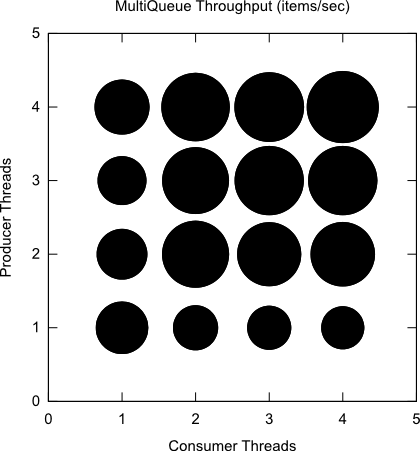
\includegraphics[width=\textwidth]{multiqueue.png}
        \caption{min=1856809, max=5150969}
    \end{subfigure}
    \hfill
    \begin{subfigure}[b]{0.45\textwidth}
        \centering
        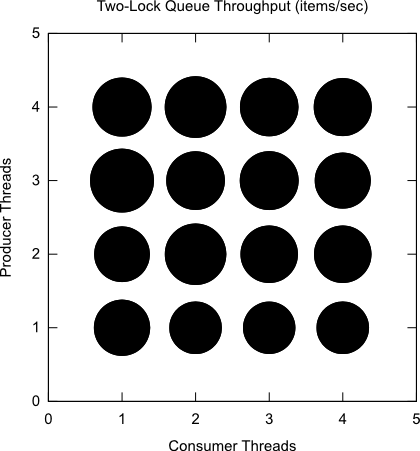
\includegraphics[width=\textwidth]{two-lock.png}
        \caption{min=2707499, max=4027409}
    \end{subfigure}
    \caption{Throughput of the queues when subjected to continuous load for 5
    seconds. The area of each circle is proportional to the throughput for a
    queue with the given number of producer and consumer threads.}
    \label{smalltest}
\end{figure}

Figure \ref{smalltest} is the result of running both the MultiQueue and the
two-lock queue for various configurations of consumers and producers. The tests
stop at four threads because the testing computer only has four cores, and
trying to scale much beyond the number of cores available produces erratic
results.

Applying the MultiQueue had the effect of moderately increasing throughput when
the number of consumers and producers are both large. Interestingly, if the
thread count for either consumers or producers is one, using the MultiQueue
causes a performance degradation.

The use of a shared counter in the MultiQueue provides a single point of
contention. Compared to the contention point offered by the head and tail locks
of the two-lock queue, the counter is a smaller penalty. Overall, there is a
trade-off between having a thread spin on a lock to perform an operation, and
having it wait on a counter to gain access to a queue. The difference is that
when a thread gains access to a queue in the MultiQueue, it is still possible
for other threads to gain access to other queues.

When there is only one consumer or one producer, the every other thread is,
essentially, waiting for that thread to complete its operation before moving
on. As a result, the likelihood of having multiple threads performing their
operations on multiple queues in parallel is small unless the one
``bottleneck'' thread performs its operation much faster than the other threads
perform theirs. It would seem the situation should not be much better than
simply using a single two-lock queue; however the lack of parallelism from the
multiple queues combined with the overhead of spinning on a shared counter
results in performance being worse than a two-lock queue under similar
conditions.

\section{Conclusion}
This paper presented a contention management system for queues called the
MultiQueue. The MultiQueue functioned by distributing the work of several
operations amongst multiple instances of the underlying concurrent queue
structure. When applied to a two-lock concurrent queue, the MultiQueue provided
a modest increase in throughput for large thread counts, and a slight
performance degradation when thread counts for either consumers or producers
were disproportionately small.

\bibliographystyle{plain}
\bibliography{report}
\end{document}
